\subsection{Piivert, a new controller}

To interact with the environment, the author developed an input device called Piivert \cite{berthaut2010piivert} shown in \ref{fig:piivert}. This device is separated in two controllers that are properly tied to each hand. That improves the musical control of the user. It combines a 6DOF tracking -that allows ray casting and some gestures detection- and high-sensitivity pressure sensing.\\
The author approach regarding the choice of musical gestures was thought following Cadoz's \cite{cadoz1999musique} research. Indeed, Cadoz suggested three categories of gestures : selection, modification and excitation gestures. As graphical interaction does not fit to the last category of gestures, the Piivert have an important part in the instrument thanks to its pressure sensing and vibrating feedback (i.e excitation can be used to trigger sequences).

\begin{figure}[h!]
\centering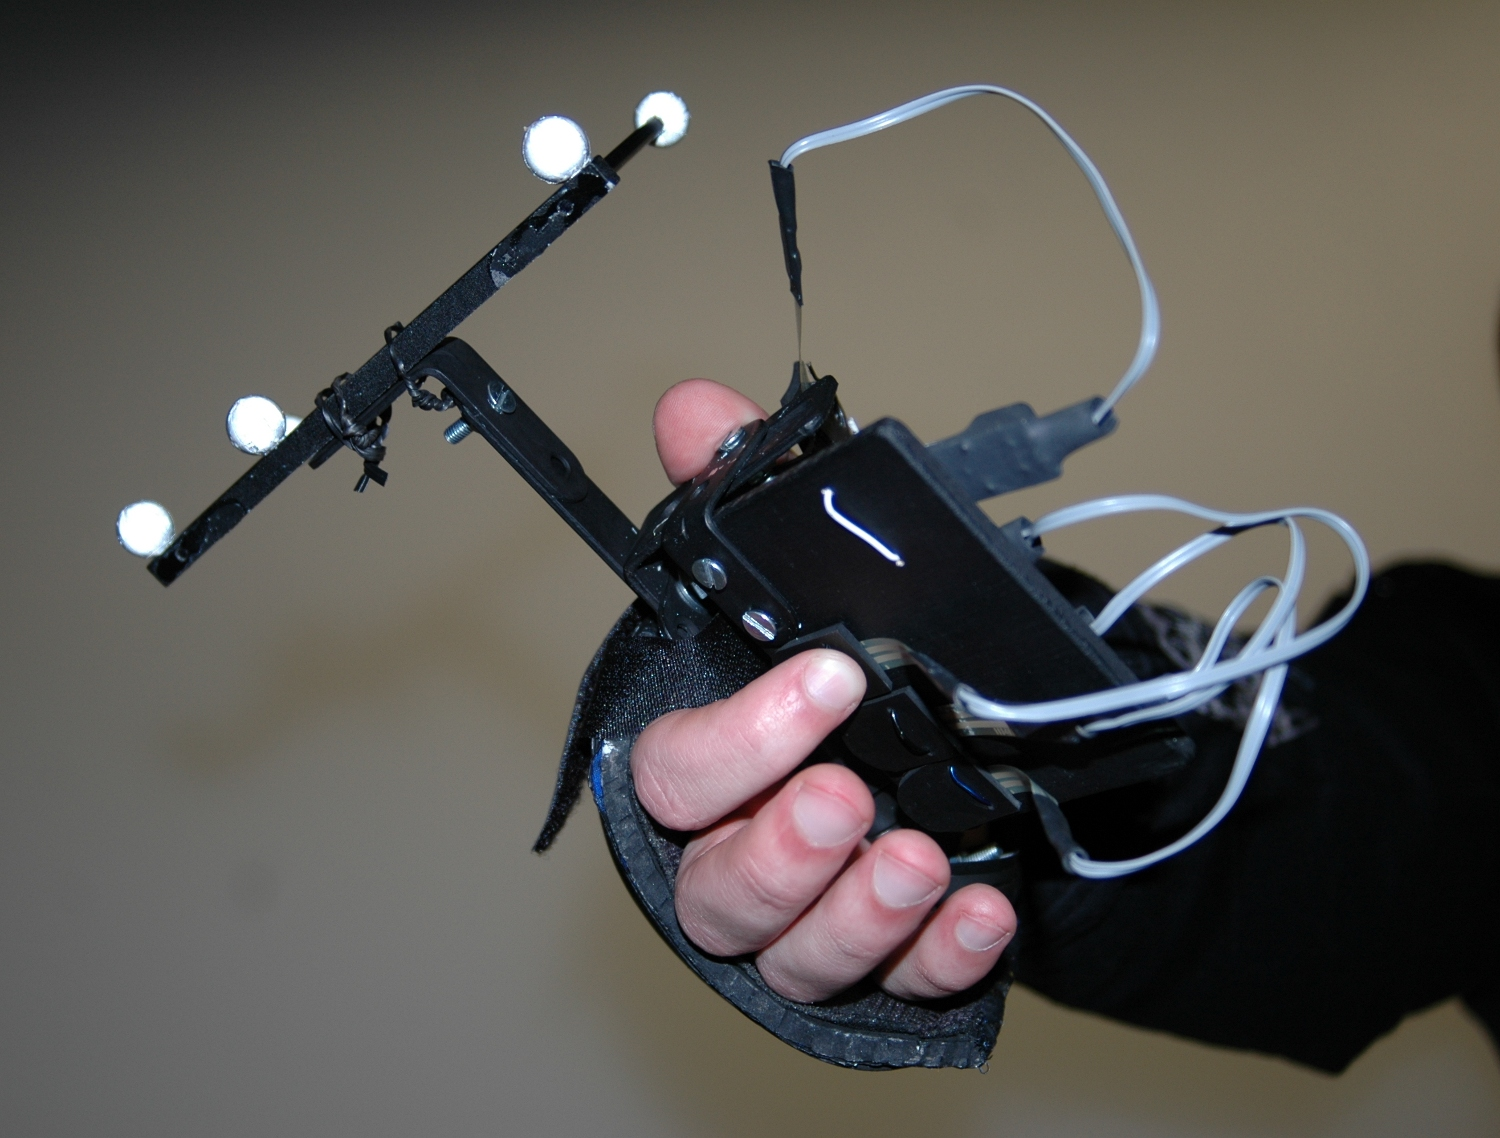
\includegraphics[width=14cm,height=4cm]{image/piivert.jpg}
\caption{Piivert with pressure buttons on the bottom}
\label{fig:piivert}
\end{figure} 